\subsection{Analysis of \acrlong{BA} model}



\subsubsection*{Classifiers for parameters based on tree shape}



Trees simulated under different values of \gls{alpha} were visibly quite
distinct (\cref{fig:alphatrees}). In particular, higher values of \gls{alpha}
produce networks with a small number of highly connected nodes which, once
infected, are likely to transmit to many other nodes. This results in a more
unbalanced, ladder-like structure in the phylogeny, compared to networks with
lower \gls{alpha} values. None of the other three parameters produced trees
which were as easily distinguished from each other
(\cref{fig:Itrees,fig:mtrees,fig:Ntrees,fig:Itrees}).  Sackin's index, which
measures tree imbalance, was significantly correlated with all four parameters
    (for $\alpha$, $I$, $m$, and $N$ respectively: Spearman's rho =
     0.85,
     \ensuremath{-0.12},
     \ensuremath{-0.13},
     0.09;
     $p$-values
     ${<}10^{-5}$,
     $0.003$,
     ${<}10^{-5}$,
     ${<}10^{-5}$)
The ratio of internal to terminal branch lengths was negatively correlated with
\gls{alpha} and \gls{I}, and positively corelated with \gls{N} and \gls{m}
  (Spearman's rho
    \ensuremath{-0.84},
    \ensuremath{-0.69},
    0.1,
    0.18;
  all $p < 10^{-5}$).

\begin{figure}[ht]
  \centering
  \includegraphics[width=\textwidth]{kernel-alpha-tree.pdf}
  \caption[Simulated transmission trees under three different values of BA parameter $\alpha$]{
    Simulated transmission trees under three different values of BA parameter
    $\alpha$. Epidemics were simulated on \gls{BA} networks of 5000 nodes, with
    \gls{alpha} equal to 0.5, 1.0, or 1.5, until 1000 individuals were
    infected. Transmission trees were created by sampling 500 infected nodes.
    Higher \gls{alpha} values produced networks with a small number of
    highly-connected nodes, resulting in highly unbalanced, ladder-like trees.
  }
  \label{fig:alphatrees}
\end{figure}

\Cref{fig:kpca} shows \gls{kPCA} projections of the simulated trees onto the
first two principal components of the kernel matrix. The figure shows only the
simulations with 500-tip trees and 1000 infected nodes. The three \gls{alpha}
and \gls{I} values considered are well separated from each other in feature
space. On the other hand, the three \gls{N} values overlap significantly, and
the three \gls{m} values are virtually indistinguishable. Similar observations
can be made for other values of \gls{I} and the number of tips
(\cref{fig:alphakpca,fig:Nkpca,fig:Ikpca,fig:mkpca}). The values of \gls{I} and
\gls{N} separated more clearly with larger numbers of tips, and in the case of
\gls{N}, larger epidemic sizes.

\begin{figure}[ht]
  \centering
  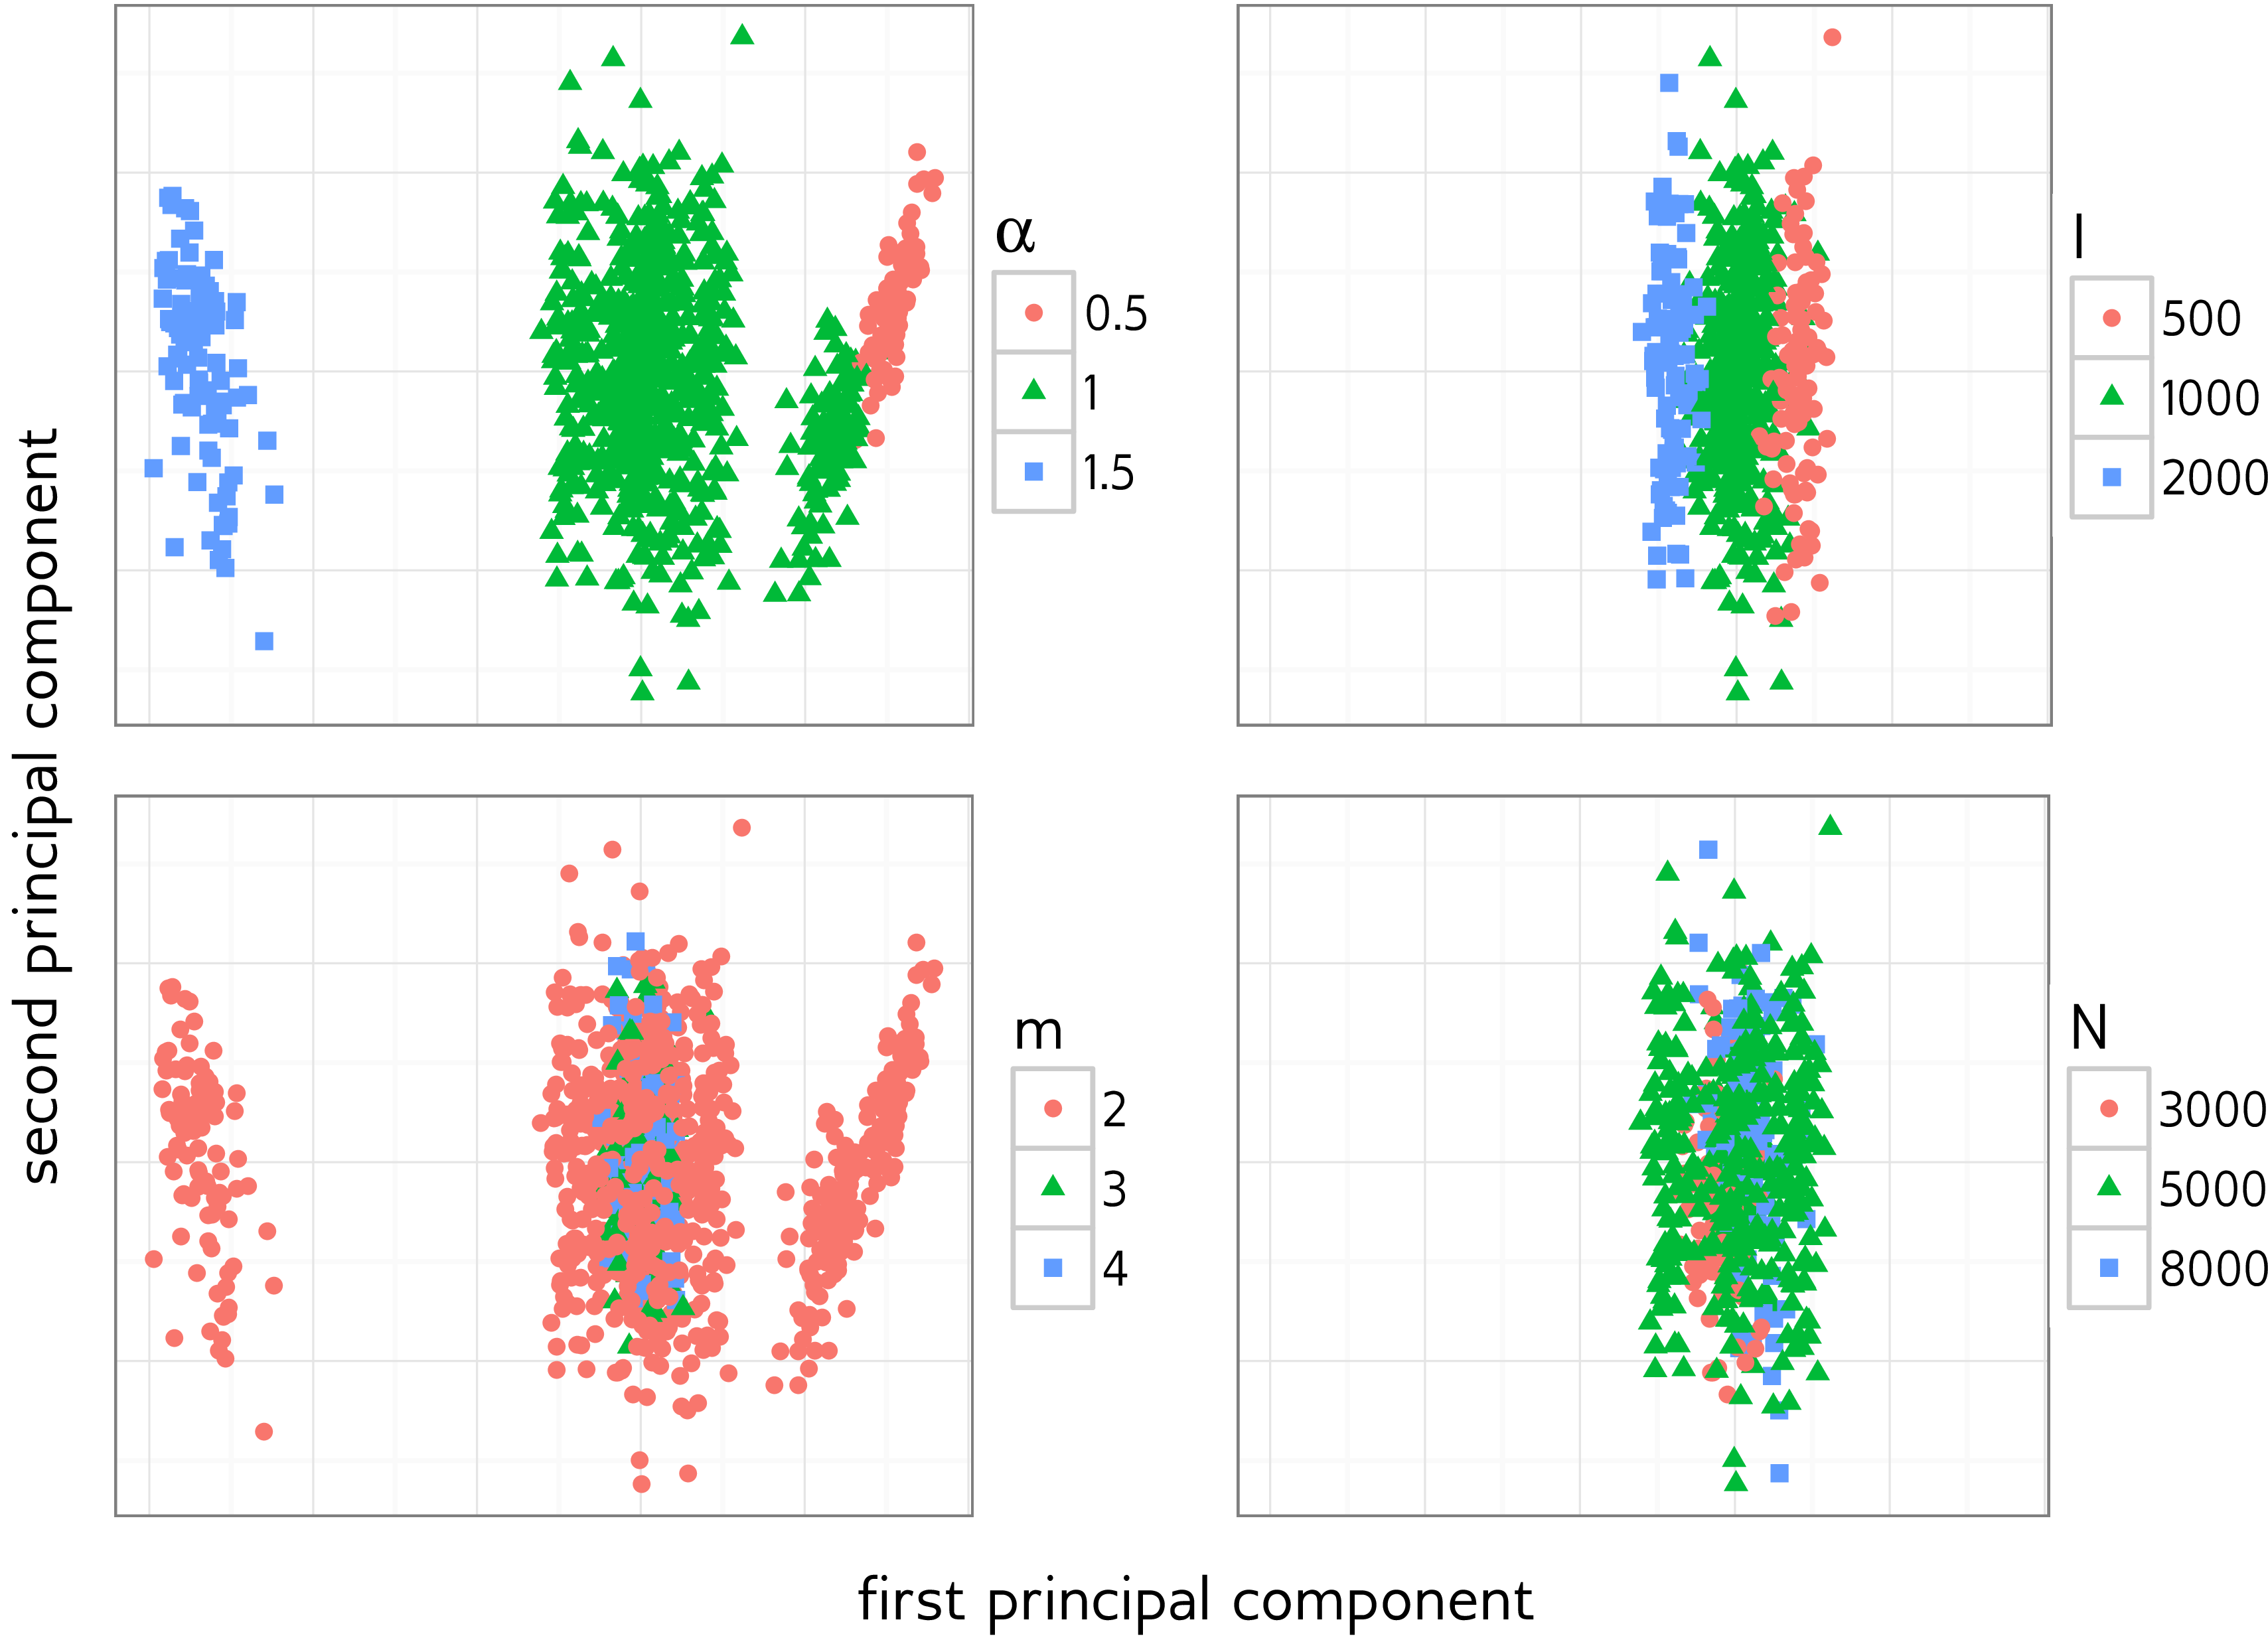
\includegraphics{kernel-kpca.pdf}
  \caption[Kernel-PCA projections of simulated trees under varying BA
           parameter values.]{
    Each parameter of the \gls{BA} model was individually varied to produce 300
    simulated trees. Kernel matrices were formed from all pairwise kernel
    scores among each set of 300 trees. The trees were projected onto the first
    two principal components of the kernel matrix calculated using \gls{kPCA}.
    All trees had 500 tips. The parameters not being varied were set to
    \gls{alpha} = 1, \gls{I} = 1000, \gls{m} = 2, and \gls{N} = 5000. The tree
    kernel meta-parameters were $\lambda = 0.3$ and $\sigma = 4$.
  }
  \label{fig:kpca}
\end{figure}



Accuracy of the \gls{kSVR} classifiers varied based on the parameter being
tested (\cref{fig:rsquared}, left). Classifiers based on two other tree
statistics, the \gls{nltt} and Sackin's index, generally exhibited worse
performance than the tree kernel, although the magnitude of the disparity
varied between the parameters (\cref{fig:rsquared}, centre and right). The
results were largely robust to variations in the tree kernel meta-parameters
$\lambda$ and $\sigma$, although accuracy varied between different epidemic and
sampling scenarios
(\cref{fig:alphacrossv,fig:mcrossv,fig:Icrossv,fig:Ncrossv}).

When classifying $\alpha$, the \gls{kSVR} classifier had an average $R^2$ of 
    0.92,
compared to 
    0.56
for the \gls{nltt}-based SVR, and
    0.75
for the linear regression against Sackin's index. There was little variation
about the mean for different tree and epidemic sizes. No classifier could
accurately identify the $m$ parameter in any epidemic scenario, with average
$R^2$ values of 
  0.12 for \gls{kSVR},
  0.01 for the \gls{nltt}, and
  0.06
for Sackin's index. Again, there was little variation in accuracy between
epidemic scenarios, although the accuracy of the \gls{kSVR} was slightly higher
on 1000-tip trees 
    (average $R^2$ 
     0.01,
     0.11,
     0.32
     for 100, 500, and 1000 tips respectively).

The accuracy of classifiers $I$ varied significantly with the number of tips in
the tree. For 100-tip trees, the average $R^2$ values were
  0.7,
  0.55, and
  0.02
for the tree kernel, \gls{nltt}, and Sackin's index respectively. For 500-tip
trees, the values increased to
  0.93,
  0.83, and
  0.07.
Finally, the performance of classifiers for $N$ depended heavily on the
epidemic scenario. The $R^2$ of the \gls{kSVR} classifier ranged from
  0.08
for the smallest epidemic and smallest sample size, to
  0.82
for the largest. Likewise, $R^2$ for the \gls{nltt}-based SVR ranged from 
  0.01
to
  0.54.
Sackin's index did not accurately classify $N$ in any scenario, with an average
$R^2$ of
  0.03
and little variation between scenarios.

\begin{figure}[ht]
  \centering
  \includegraphics[width=\textwidth]{kernel-rsquared.pdf}
  \caption[Cross-validation accuracy of kernel-SVR, nLTT-based SVR, and
  Sackin's index regression classifiers for BA model parameters.]{
      Cross-validation accuracy of kernel-SVR classifier (left), SVR classifier
      using \gls{nltt} (centre), and linear regression using Sackin's index
      (right) for \gls{BA} model parameters. Kernel meta-parameters were set to
      $\lambda = 0.3$ and $\sigma = 4$. Each point was calculated based on 300
      simulated transmission trees over networks with three different values of
      the parameter being tested. Vertical lines are empirical 95\% confidence
      intervals based on 1000 two-fold cross-validations.
  }
  \label{fig:rsquared}
\end{figure}

\subsubsection*{Marginal parameter estimates with grid search}



The accuracy of grid search estimates largely paralleled that of the \gls{kSVR}
classifiers. \Cref{fig:gridest} shows point estimates and 95\% highest density
intervals for each of the \gls{BA} parameters, for one replicate experiment
with 500-tip trees. Plots showing the point estimates for all replicates can be
found in \cref{fig:gridptalpha,fig:gridptI,fig:gridptm,fig:gridptN}. For all
parameters except $m$, the error of point estimates was negatively correlated
with the number of sampled tips in the tree (for
\gls{alpha}, \gls{I}, and \gls{N} respectively: Spearman's $\rho$ = 
    \ensuremath{-0.22},
    \ensuremath{-0.51},
    \ensuremath{-0.16};
$p$-values
    $4\!\times\!10^{-4}$,
    ${<}10^{-5}$,
    $0.01$).
The highest density intervals obtained for all parameters were extremely wide,
occcupying $>$90\% of the grid in all cases (\cref{fig:gridest}).

The \gls{alpha} parameter was the most accurately estimated, with point
estimates having an average deviation of 
    0.14
from the true value, on a grid from 0 to 2. The error was negatively correlated
with the true value of \gls{alpha} 
    (Spearman's $\rho$ = \ensuremath{-0.26},
     $p = 10^{-5}$),
although the relationship was clearly nonlinear (\cref{fig:gridest,fig:gridalpha}).
The accuracy was highest for the test value \gls{alpha} = 1.25
    (mean error 0.02)
which exhibited markedly different behaviour than the other values in terms of
the distribution of kernel scores along the grid (\cref{fig:gridalpha}). In
particular, there was a very pronounced peak in scores around the true value,
in contrast to most other values where the scores were flat around the true
value. The peak was also observed to a lesser degree for \gls{alpha} = 1. The
average absolute error of the point estimates for \gls{I} was 
    310,
on a grid of 500 to 5000, and the errors were not significantly correlated with
the true value of \gls{I}. Kernel score distributions for all test values
exhibited a similar rounded shape (\cref{fig:gridI}). 

The average error for \gls{m} was
    1.31,
on a grid from 1 to 6; this error was positively correlated with increasing
\gls{m}
    (Spearman's $\rho$ = 0.25,
     $p = 6\!\times\!10^{-4}$).
This positive correlation was apparently due to the much lower error for
\gls{m} = 1 and 2 than for the other $m$ values 
    (mean errors 
    0.93 
    for $m \leq 2$ vs. 
    1.49 
    for $m > 2$, \cref{fig:gridm}).
The value $m = 1$ causes the network to take on a distinct shape relative to
higher \gls{m} values, namely a tree (\textit{i.e.} there are no cycles,
see \cref{subsec:treeshape}). The average error for \gls{N} was 
    2419,
on a grid from 1000 to 15000, and was positively correlated with the true value
of \gls{N}
    (Spearman's $\rho$ = 0.43,
    $p\ {<}10^{-5}$). 
Most of the kernel score distributions were extremely flat, except for the
value $N = 1000$ which exhibited a pronounced peak around the true value
(\cref{fig:gridN}).

\begin{figure}[ht]
  \centering
  \includegraphics[width=\textwidth]{gridsearch-example}
  \caption[Grid search estimates of \gls{BA} model parameters.]{Point estimates
      and 95\% highest density intervals for each \gls{BA} model parameter,
      obtained using grid search. Networks and transmission trees were
      simulated over a grid of values for each parameter while holding the
      others fixed. For a subset of the grid values ($x$-axis), test networks
      and trees were created and compared to each tree on the grid using the
      tree kernel. The kernel scores along the grid were normalized to resemble
      a probability distribution, from which the mode and highest density
      interval were calculated. Shown values correspond to one replicate
      experiment, with trees of size 500.
  } 
  \label{fig:gridest}
\end{figure}

\subsubsection*{Joint parameter estimates with kernel-ABC}



We used \software{netabc} to estimate the parameters of the \gls{BA} model on
simulated trees where the true parameter values were known. Point estimates for
each parameter are shown in \cref{fig:abcptm2} for the simulations with \gls{m} =
2. The results for the other values of \gls{m} were similar
(\cref{fig:abcptm3,fig:abcptm4}). The median [IQR] absolute error of estimates of
\gls{alpha} across all simulations was
    0.08 
    [0.05-0.17].
The accuracy of the estimates was not significantly different between values of
$m$ or $I$ (both one-way ANOVA,
    $p$ = 0.05
and 
    0.07),
although the errors when the true value of \gls{alpha} was zero were
significantly greater than the other values 
    (Wilcoxon rank-sum test, $p = 8\!\times\!10^{-3}$).
The error in the estimated value of $I$ was
    395 
    [207-683].
Errors were significantly higher for $\alpha \geq 1$
    (Wilcoxon rank-sum test, $p = 8\!\times\!10^{-3}$)
and for $I$ = 2000
    ($p = {<}10^{-5}$),
but not for any values of $m$ (one-way ANOVA). The $m$ parameter was estimated
correctly in only
    27 \%
of simulations, little better than random guessing. The true values of $m$ and
$I$ did not significantly affect the error (one-way ANOVA). Finally, the total
number of nodes \gls{N} was consistently over-estimated by about a factor of
two
    (error 5987 
    [2060 - 
     7999]).
No other parameters influenced the accuracy of the $N$ estimates (one-way
ANOVA).

\begin{figure}
  \includegraphics{abc-point-estimate-m2}
  \caption[\Acrlong{MAP} point estimates for \gls{BA} model parameters obtained
    by running \software{netabc} on simulated data, for simulations with $m = 2$.] 
  {
    \Acrlong{MAP} point estimates for \gls{BA} model parameters obtained by         
    running \software{netabc} on simulated data. Values shown are for               
    simulations with \gls{m} = 2. Dashed lines indicate true values. (A)            
    Estimates of \gls{alpha} and \gls{I} which were varied in these simulations  
    against known values. (B) Estimates of \gls{m} and \gls{N} which were held   
    fixed in these simulations at the values \gls{m} = 2 and \gls{N} = 5000. 
  }
  \label{fig:abcptm2}
\end{figure}



\Cref{fig:abcex} shows the \gls{ABC} approximation to the posterior
distribution on the \gls{BA} parameters for one simulation. Equivalent plots
for one replicate simulation with each combination of parameters can be found
in \cref{fig:0.0-1000-2-5000-0,fig:0.5-1000-2-5000-0,fig:1.0-1000-2-5000-0,fig:1.5-1000-2-5000-0,fig:0.0-2000-2-5000-0,fig:0.5-2000-2-5000-0,fig:1.0-2000-2-5000-0,fig:1.5-2000-2-5000-0,fig:0.0-1000-3-5000-0,fig:0.5-1000-3-5000-0,fig:1.0-1000-3-5000-0,fig:1.5-1000-3-5000-0,fig:0.0-2000-3-5000-0,fig:0.5-2000-3-5000-0,fig:1.0-2000-3-5000-0,fig:1.5-2000-3-5000-0,fig:0.0-1000-4-5000-0,fig:0.5-1000-4-5000-0,fig:1.0-1000-4-5000-0,fig:1.5-1000-4-5000-0,fig:0.0-2000-4-5000-0,fig:0.5-2000-4-5000-0,fig:1.0-2000-4-5000-0,fig:1.5-2000-4-5000-0}. \Gls{HPD} intervals around \gls{alpha} and \gls{I} were
narrow relative to the region of nonzero prior density, whereas the intervals
for $m$ and \gls{N} were widely dispersed. \Cref{tab:abchpd} shows point
estimates and 95\% \gls{HPD} intervals averaged over all simulations.

\begin{figure}
  \includegraphics{{abc-posterior/1.0_1000_2_5000_0}.pdf}
  \caption[Approximate marginal posterior distributions of BA model parameters
      obtained by applying \textit{netabc} to a simulated transmission tree
      with values $\alpha$ = 1.0, $I$ = 1000, $m$ = 2, and $N$ = 5000.]
    {
        Approximate marginal posterior distributions of BA model parameters
        obtained by applying \textit{netabc} to a simulated transmission tree
        with BA parameter values $\alpha$ = 1.0, $I$ = 1000, $m$ = 2, and $N$ =
        5000. Vertical dashed lines indicate true values. Shaded areas are 95\%
        highest posterior density intervals. $x$-axes indicate regions of
        nonzero prior density.
    }
  \label{fig:abcex}
\end{figure}


\begin{table}
    \centering
    % latex table generated in R 3.2.3 by xtable 1.8-2 package
% Fri Jun 17 12:51:45 2016
\begin{tabular}{lr>{\raggedleft\arraybackslash}p{2.5cm}>{\raggedleft\arraybackslash}p{2.5cm}>{\raggedleft\arraybackslash}p{2.5cm}}
  \hline
Parameter & True value & Mean point estimate & Mean HPD lower bound & Mean HPD upper bound \\ 
  \hline
$\alpha$ & 0.0 & 0.36 & 0.01 & 0.81 \\ 
   & 0.5 & 0.43 & 0.04 & 0.83 \\ 
   & 1.0 & 0.90 & 0.51 & 1.09 \\ 
   & 1.5 & 1.52 & 1.26 & 1.81 \\ 
  $I$ & 1000 & 1450 & 651 & 2592 \\ 
   & 2000 & 2622 & 1114 & 4080 \\ 
  $m$ & 2 & 2.96 & 2.00 & 5.00 \\ 
   & 3 & 3.04 & 2.04 & 4.96 \\ 
   & 4 & 3.17 & 1.88 & 5.00 \\ 
  $N$ & 5000 & 9041 & 2613 & 14659 \\ 
   \hline
\end{tabular}

    \caption[
        Maximum \textit{a priori} estimates and 95\% highest posterior density
        (HPD) interval boundaries for \gls{BA} model parameters estimated with
        \software{netabc}, averaged over simulated transmission trees.
    ]
    {
        Maximum \textit{a priori} estimates and 95\% highest posterior density
        (HPD) interval boundaries for \gls{BA} model parameters estimated with
        \software{netabc}, averaged over simulated transmission trees.
    }
    \label{tab:abchpd}
\end{table}



To test the effect of model misspecification, we simulated one network where
the nodes exhibited heterogeneous preferential attachment power (half 0.5, the
other half 1.5), with $m$ = 2, $N$ = 5000, and $I$ = 1000. The MAP [95\%
HPD] estimates for each parameter were: 
$\alpha$, 
  1.1 
  [0.6 -
   1.16];
$I$,
  1091 
  [662 -
   4455];
$m$,
  3 
  [1 -
   5];
$N$,
  12566 
  [3733 -
   14945].
The approximate posterior distributions for this simulation are shown in
\cref{fig:mixed}. To test the effect of sampling bias, we sampled one
transmission tree in a peer-driven fashion, where the probability to sample a
node was twice as high if one of its peers had already been sampled. The
parameters for this experiment were $N$ = 5000, $m$ = 2, $\alpha$ = 0.5, and
$I$ = 2000. The estimated values were
$\alpha$, 
  0.37 
  [0 -
   0.62];
$I$,
  2407 
  [1423 -
   3811];
$m$,
  3 
  [2 -
   5];
$N$,
  13811 
  [2624 -
   14647].
The approximate posterior distributions are shown in \cref{fig:peerdriven}. Both
of these results were in line with estimates obtained on other simulated
datasets (\cref{tab:abchpd}), although the estimate of peer-driven sampling for
$\alpha$ was somewhat lower than typical.

%\subsubsection*{Effect of parameters on power-law exponent}
%
%\Cref{tab:glm} shows the estimated parameters for a log-link \gls{GLM} fitted
%to the observed distribution of \gls{gamma} values. The coefficients are
%interpretable as multiplicative effects.
%
%\begin{table}
%    \centering
%    % latex table generated in R 3.2.3 by xtable 1.8-2 package
% Tue Mar 15 09:15:55 2016
\begin{tabular}{rrrl}
  \hline
 & exp(Estimate) & Standard error & P-value \\ 
  \hline
(Intercept) & 1.63 & $5.1 \times 10^{-3}$ & $<10^{-5}$ \\ 
  $\alpha$ & 1.77 & $4.4 \times 10^{-3}$ & $<10^{-5}$ \\ 
  $m$ & 1.03 & $1.0 \times 10^{-3}$ & $<10^{-5}$ \\ 
  $N$ & 1.00 & $5.8 \times 10^{-7}$ & $<10^{-5}$ \\ 
  $\alpha \times m$ & 1.00 & $8.7 \times 10^{-4}$ & $<10^{-5}$ \\ 
  $\alpha \times N$ & 1.00 & $5.0 \times 10^{-7}$ & $<10^{-5}$ \\ 
  $m \times N$ & 1.00 & $1.1 \times 10^{-7}$ & $<10^{-5}$ \\ 
  $\alpha \times m \times N$ & 1.00 & $9.9 \times 10^{-8}$ & $<10^{-5}$ \\ 
   \hline
\end{tabular}

%    \caption{Estimated \gls{GLM} parameters for relationship between power-law
%    exponent \gls{gamma} and \gls{BA} model parameters.}
%    \label{tab:glm}
%\end{table}

\subsection{Application to HIV data}



We applied kernel-ABC to five published HIV datasets (\cref{tab:data}),
and found substantial heterogeneity among the parameter estimates
(\cref{fig:abchpd,fig:abchpdm2}). Plots of the marginal posterior distributions
for each dataset are shown in
\cref{fig:cuevas,fig:li,fig:niculescu,fig:novitsky,fig:wang}.
Two of the datasets (\textcite{niculescu2015recent, wang2015targeting}) had
estimated $\alpha$ values near unity for the prior allowing $m = 1$ (\gls{MAP}
estimates [95\% \gls{HPD}] 
  1.05 
  [0.04 - 
   1.27]
and
  0.84 
  [0.01 -
   1.02] respectively).
The MAP estimates did not change appreciably when $m = 1$ was disallowed by the
prior, although the credible interval of the \textcite{niculescu2015recent}
data was narrower
  (0.04 - 
   1.27).
When $m = 1$ was permitted, the \textcite{li2015hiv, cuevas2009hiv} both had
low estimated $\alpha$ values
  (0.06 
  [0.01 - 
  0.73]
and
  0.19 
  [0.01 -
   0.8]). 
However, the MAP estimates increased when $m = 1$ was not permitted, although
the HPD intervals remained roughly the same
  (0.78 
  [0.02 - 
  0.94]
and
  0.59 
  [0.07 -
   0.95]).
The \textcite{novitsky2014impact} data had a fairly low estimated $\alpha$
for both priors on $m$
  (0.32 for $m \geq 1$;
   0.39 for $m \geq 2$).
However, the confidence interval was much wider when $m = 1$ was allowed
  ([0.04 -
    1.62] for $m \geq 1$ vs.
   [0 -
    0.73] for $m \geq 2$).

For all the datasets except \citeauthor{novitsky2014impact}, estimated values
of $I$ were below 2000 when $m = 1$ was allowed, with relatively narrow HPD
intervals compared to the nonzero prior density region
  (\citeauthor{cuevas2009hiv}, 482 
  [293 -
   2111];
   \citeauthor{niculescu2015recent}, 307
  [136 - 
   2822];
  \citeauthor{li2015hiv}, 1183 
  [413 -
   2897];
   \citeauthor{wang2015targeting}, 719
  [176 - 
   2114]).
The \citeauthor{novitsky2014impact} data was the outlier, with a very high
estimated $I$, and HPD interval spanning almost the entire prior region
  (7409 
  [187 -
   8819]).
The $I$ estimates and HPD intervals were generally robust to the choice of
prior on $m$, with slightly narrower HPD intervals (compare
\cref{fig:abchpd,fig:abchpdm2}).

The MAP estimate of $m$ was equal to 1 for all but the
\citeauthor{novitsky2014impact} data, when this value was allowed. However, the
upper bound of the HPD interval was different for each dataset
  (\citeauthor{niculescu2015recent}, 5;
   \citeauthor{wang2015targeting}, 4;
   \citeauthor{li2015hiv}, 1;
   \citeauthor{cuevas2009hiv}, 2).
When $m = 1$ was disallowed, the MAP for all datasets was either 2 or 3, with
HPD intervals spanning the entire prior region. The estimates for the total
number of nodes $N$ were largely uninformative for all samples, with almost all
MAP estimates greater than 7500 and HPD intervals spanning almost the entire
nonzero prior density region. The only exception was the \citeauthor{li2015hiv}
data, for which the MAP estimate was lower 
  (6973)
when $m = 1$ was allowed.

\begin{figure*}[ht]
  \centering
  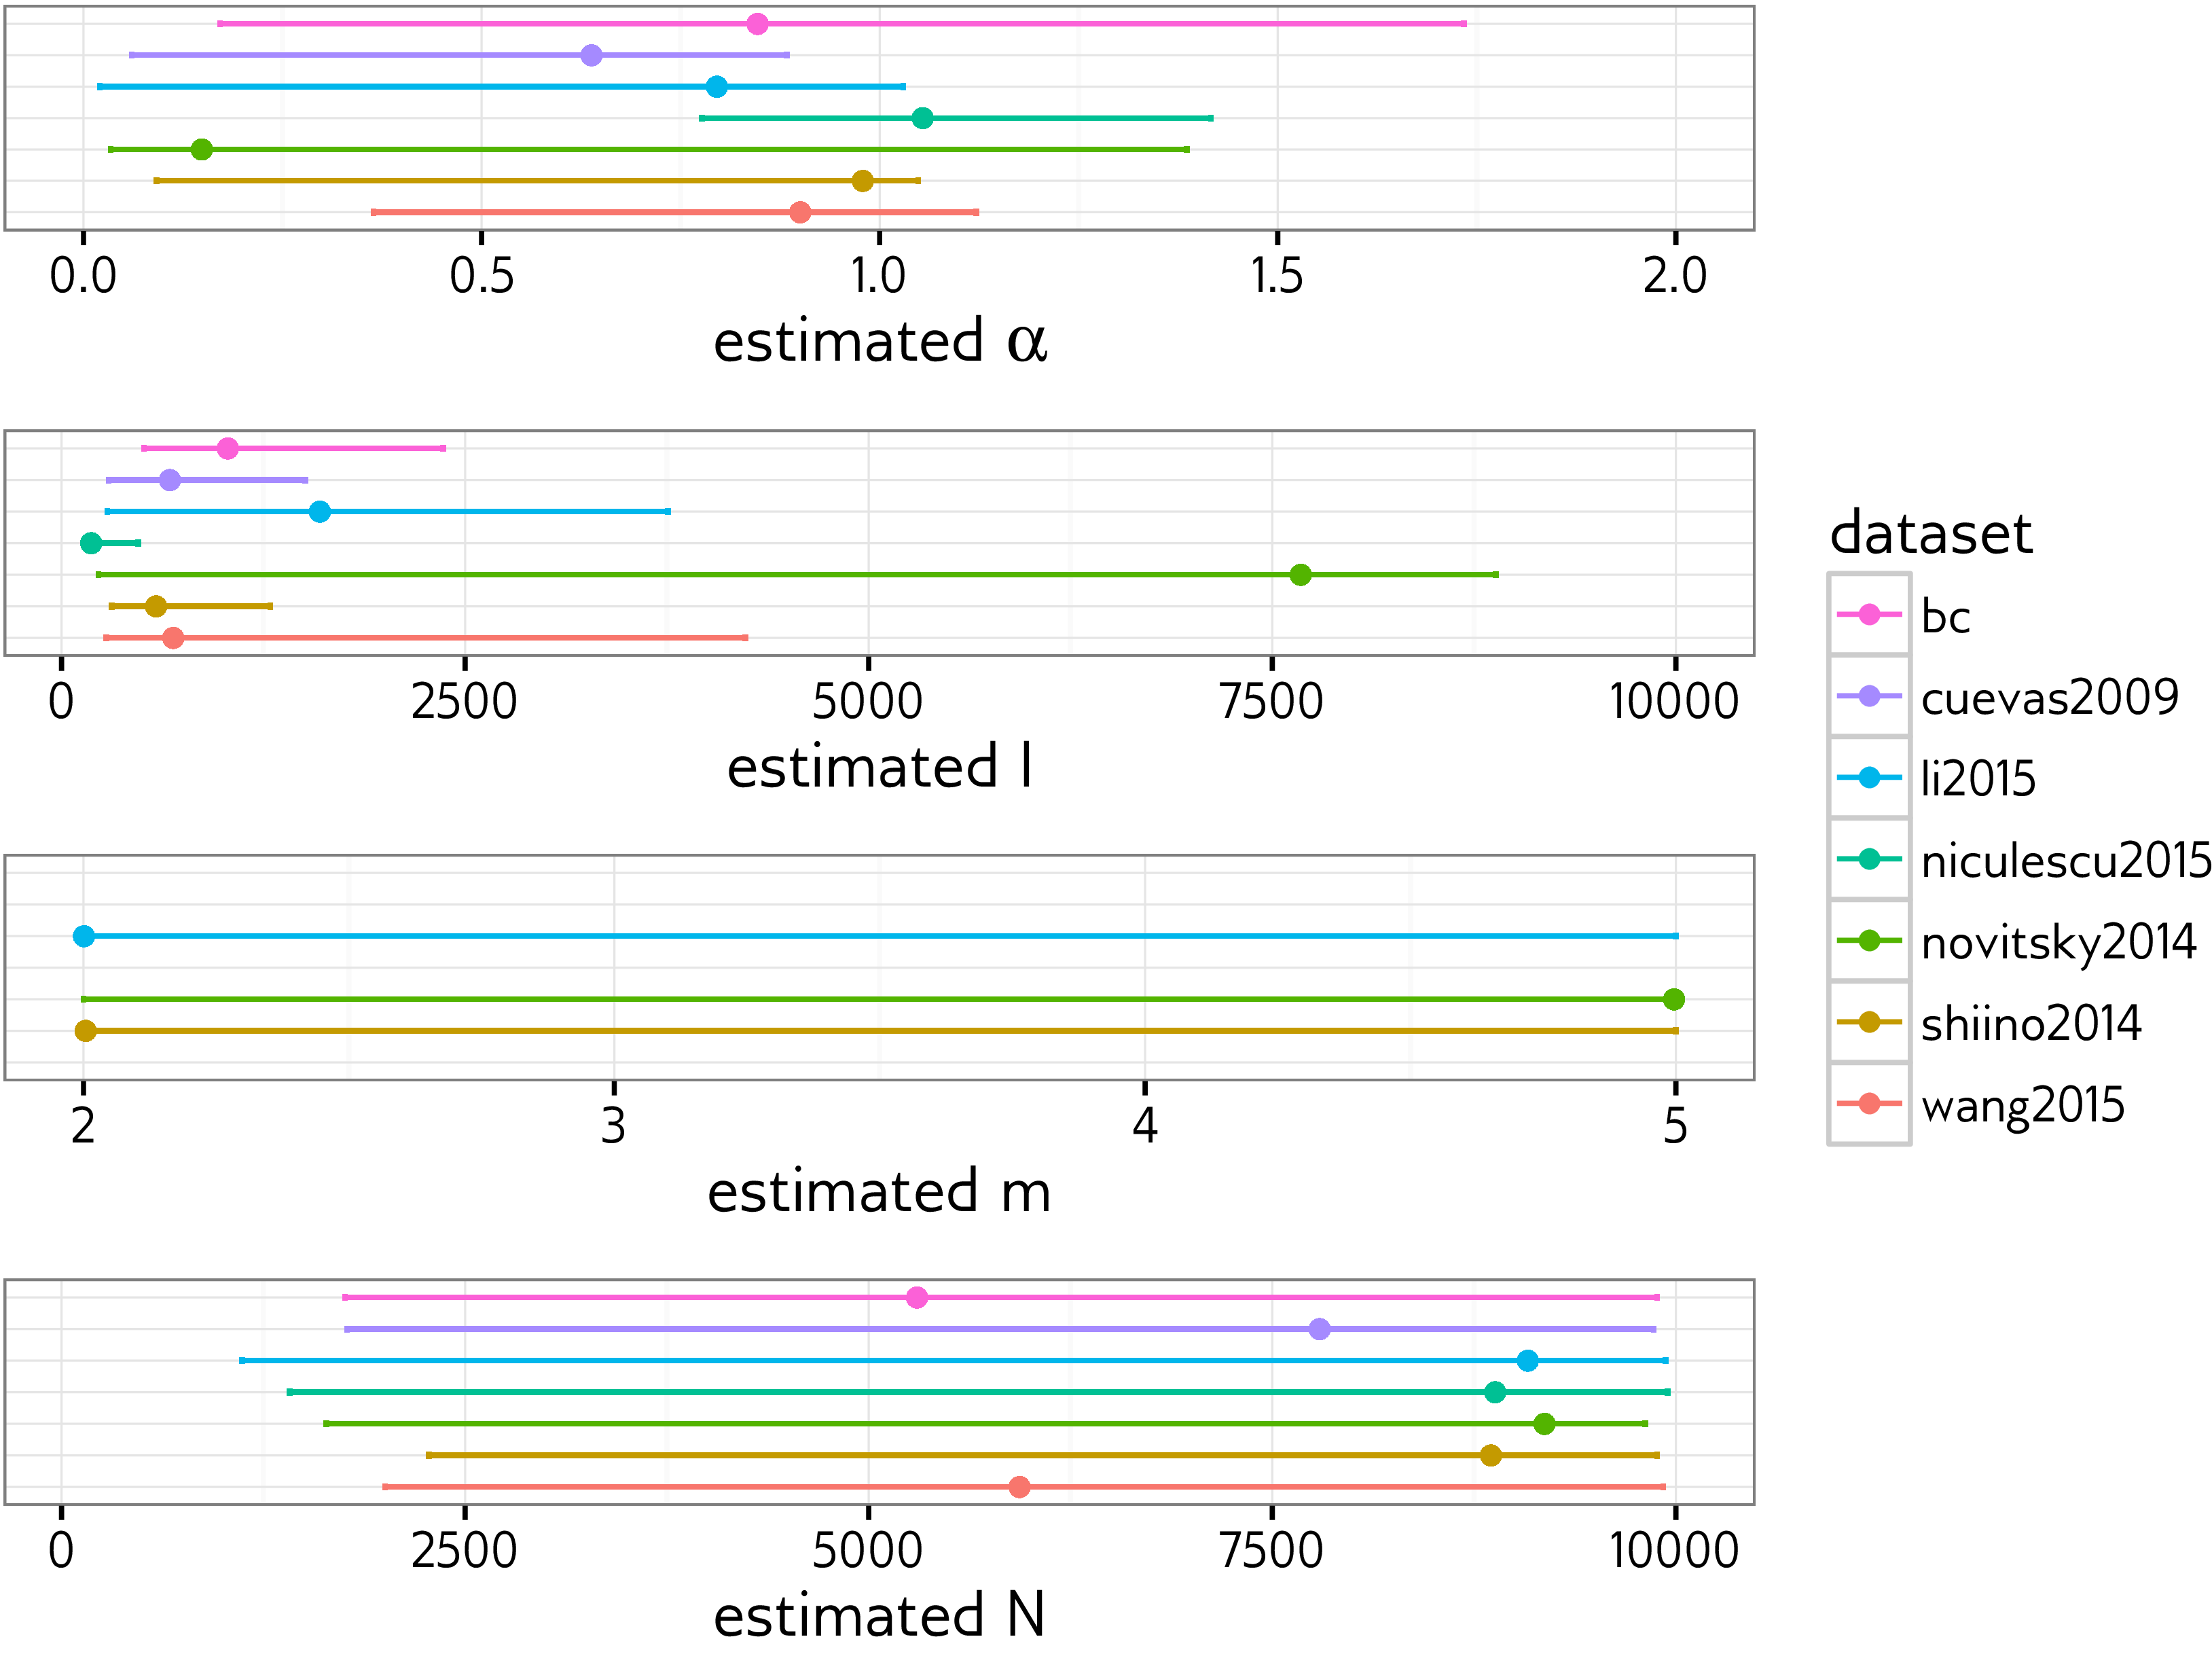
\includegraphics{realdata-hpd-bc}
  \caption[
      Maximum \textit{a posteriori} point estimates and 95\% HPD intervals for
      parameters of the BA network model, fitted to six HIV datasets
      with \software{netabc}.]
  {
      Maximum \textit{a posteriori} point estimates and 95\% HPD intervals for
      parameters of the BA network model, fitted to six HIV datasets with
      \software{netabc}. Legend labels indicate risk group and country of
      origin. Abbreviations: IDU, injection drug users; MSM, men who have sex
      with men; HET, heterosexual.
  }
  \label{fig:abchpd}
\end{figure*}
